\documentclass[tikz,border=5pt]{standalone}

\usepackage{amsmath}
\usepackage{tikz}
\usetikzlibrary{arrows.meta, positioning}

\begin{document}

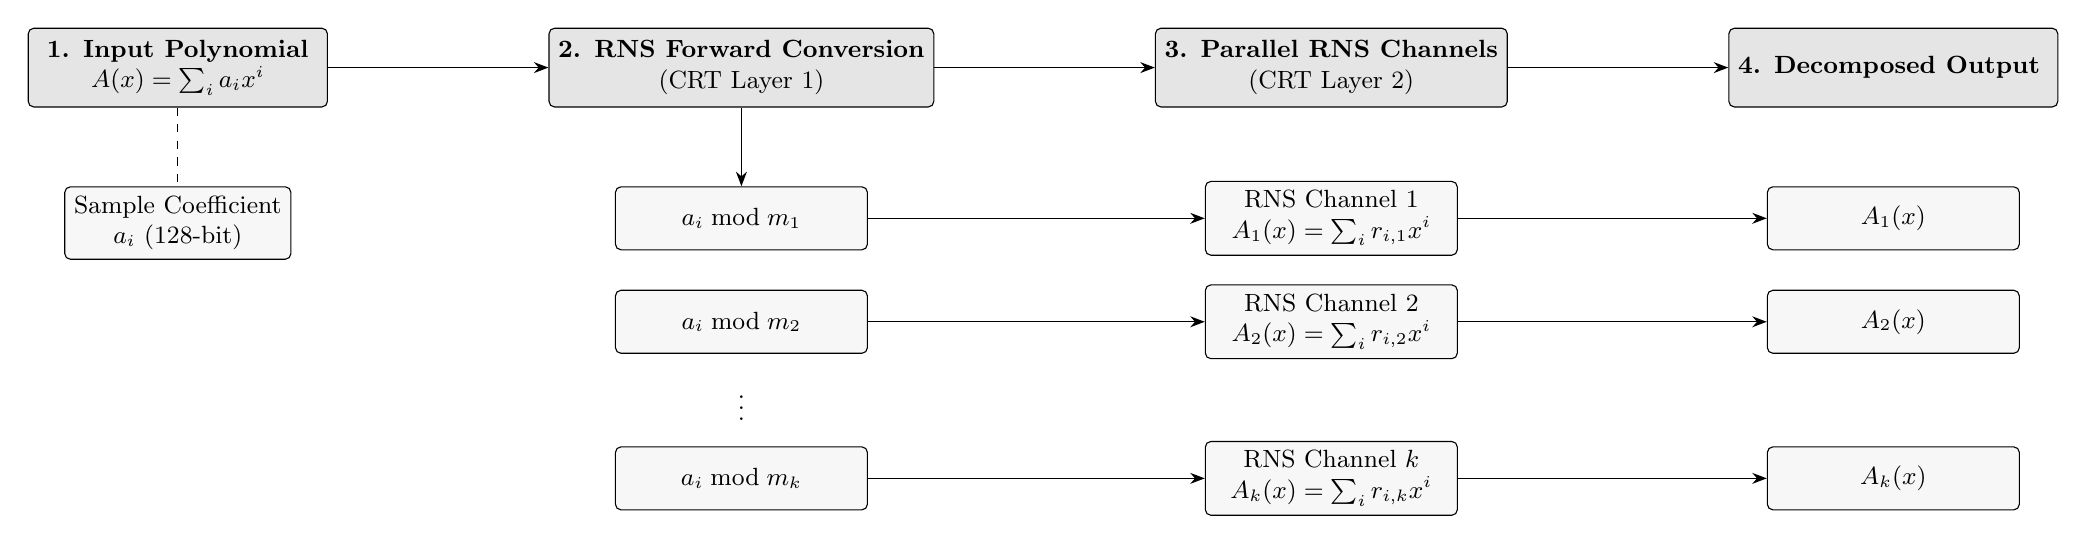
\begin{tikzpicture}[
    stage/.style={
        draw, fill=black!10,
        rectangle, rounded corners=2pt,
        minimum height=1.0cm, minimum width=3.8cm,
        align=center, font=\small
    },
    detail/.style={
        draw, fill=black!3,
        rectangle, rounded corners=2pt,
        minimum height=0.8cm, minimum width=3.2cm,
        align=center, font=\small
    },
    dataflow/.style={->, >=Stealth, line width=0.5pt},
    struct/.style={dashed, line width=0.4pt},
]

% Top row: pipeline stages
\node[stage] (stage1) {%
    \textbf{1. Input Polynomial}\\
    $A(x)=\sum_i a_i x^i$
};

\node[stage, right=2.8cm of stage1] (stage2) {%
    \textbf{2. RNS Forward Conversion}\\
    (CRT Layer 1)
};

\node[stage, right=2.8cm of stage2] (stage3) {%
    \textbf{3. Parallel RNS Channels}\\
    (CRT Layer 2)
};

\node[stage, right=2.8cm of stage3] (stage4) {%
    \textbf{4. Decomposed Output}
};

% Stage 1 detail
\node[detail, below=1.0cm of stage1, minimum width=2.8cm] (coeff) {%
    Sample Coefficient\\
    $a_i$ (128-bit)
};

\draw[struct] (stage1.south) -- (coeff.north);

% Stage 2 detail
\node[detail, below=1.0cm of stage2] (mod1) {$a_i \bmod m_1$};
\node[detail, below=0.5cm of mod1] (mod2) {$a_i \bmod m_2$};
\node[below=0.2cm of mod2, font=\small] (dots) {$\vdots$};
\node[detail, below=0.2cm of dots] (modk) {$a_i \bmod m_k$};

\draw[dataflow] (stage2.south) -- (mod1.north);

% Stage 3 detail: x from stage3, y from mod row (|- syntax)
\node[detail] (ch1) at (stage3 |- mod1) {%
    RNS Channel 1\\
    $A_1(x)=\sum_i r_{i,1} x^i$
};

\node[detail] (ch2) at (stage3 |- mod2) {%
    RNS Channel 2\\
    $A_2(x)=\sum_i r_{i,2} x^i$
};

\node[detail] (chk) at (stage3 |- modk) {%
    RNS Channel $k$\\
    $A_k(x)=\sum_i r_{i,k} x^i$
};

\draw[dataflow] (mod1.east) -- (ch1.west);
\draw[dataflow] (mod2.east) -- (ch2.west);
\draw[dataflow] (modk.east) -- (chk.west);

% Stage 4 detail: x from stage4, y from ch row
\node[detail] (out1) at (stage4 |- ch1) {$A_1(x)$};
\node[detail] (out2) at (stage4 |- ch2) {$A_2(x)$};
\node[detail] (outk) at (stage4 |- chk) {$A_k(x)$};

\draw[dataflow] (ch1.east) -- (out1.west);
\draw[dataflow] (ch2.east) -- (out2.west);
\draw[dataflow] (chk.east) -- (outk.west);

% Top-level data flow
\draw[dataflow] (stage1) -- (stage2);
\draw[dataflow] (stage2) -- (stage3);
\draw[dataflow] (stage3) -- (stage4);

\end{tikzpicture}

\end{document}
